\documentclass{article}

\usepackage{standalone}
\usepackage{pgfplots}
\pgfplotsset{compat=newest}
\usepackage{tikz}
\usetikzlibrary{decorations.markings}
\usetikzlibrary{patterns}

\usepackage{subcaption}
\usepackage[margin=2.5cm]{geometry}
\usepackage{amsmath}
\usepackage{amssymb}


\newcommand\greybox[1]{
	\vskip\baselineskip
	\par\noindent\colorbox{lightgray}{
		\begin{minipage}{\textwidth}#1\end{minipage}
	}
	\vskip\baselineskip
}

\title{En-dimensionale potensialer}


\begin{document}
\maketitle


Vi skal i dette kapitelet se på en rekke forskjellige en-dimensionale potensialer, som vi løser
S.L. for og finner bølgefunksjonene til, og ser på tolkninger av.

\section*{Partikkel i brønn}
Vi skal nå se på en partikkel som befinner seg i en potensial-brønn. Dette er beskrevet av 
potensialet 
\begin{align}
	 V(x) = \begin{cases}
		0 \hspace{0.75cm} |x| < \frac{a}{2} \\
		V_0 \hspace{.625cm} |x| \ge \frac{a}{2} 
		\end{cases}
\end{align}
Dette ligner partikkel i boks scenarioet vi så tidligere, men her er ikke potensialet uendelig 
stort utenfor boksen, slik at partikkelen kan befinne seg der også.

\begin{figure}[h!]
     \centering
     \begin{subfigure}[b]{0.4\linewidth}
       \centering
	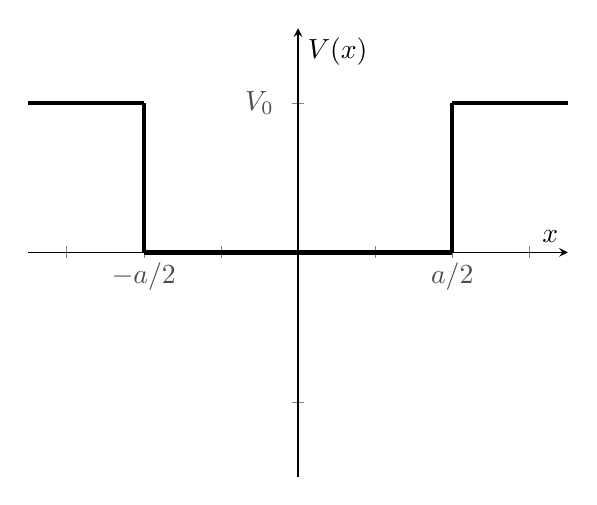
\begin{tikzpicture}
	  \begin{axis}%
	    [
	     xlabel=$x$,
	     ylabel=$V(x)$,
	     axis lines=middle,
	     restrict y to domain=-1:2.,
	     enlargelimits={abs=.75},
	     yticklabels=\empty,
	     xticklabels=\empty
	    ]
	    \addplot+[mark=none, 
		    domain=-1:1,
		    samples=150,
		    draw=black!70,
		    pattern color=black,
	    	    area legend] { 0 }  ;
	    \node [color=black!70] at (-0.25, 0.5) {$V_0$};
	    \node [color=black!70] at (1, -0.08) {$a /2$};
	    \node [color=black!70] at (-1, -0.08) {$-a /2$};
	\draw [ultra thick] (1, 0.5) -- (2,0.5);
	\draw [ultra thick] (-1, 0.5) -- (-2,0.5);
	\draw [ultra thick] (1, 0) -- (1,0.5);
	\draw [ultra thick] (-1, 0) -- (-1,0.5);
	\draw [ultra thick] (-1, 0) -- (1,0);
	  \end{axis}
	\end{tikzpicture}
         \label{fig:cos}
     \end{subfigure}
       \caption{Potensialet $V(x)$ til partikkel-brønn.}
        \label{fig:bølger}
\end{figure}
Vi løser nå S.L. for dette potensialet ved å dele opp problemet i flere områder.
Vi ser på løsningene for $|x|<a /2$, $x>a/2$ og $x<-a /2$ hver for seg og 
bruker randbetingelser for å fuge de sammen til en koherent bølgefunksjon. 
Vi skal også begrense oss til å se på bølgefunksjoner som har energi mindre enn $V_0$.
For hver av de tre tilfellene får vi essensielt en fri-partikkel S.L. som vi må løse.
Vi minner oss på at vi har den tidsuavhengige S.L. som
\begin{align}
	 \frac{-\hbar^2}{2m} \frac{\partial^2 \psi}{\partial x^2} + V(x)\psi  = E\psi
\end{align}
Vi starter med $|x|<a$, hvor vi har 
\begin{align}
	 \frac{\partial^2 \psi}{\partial x^2}  = -k^2\psi
\end{align}
hvor $k=\sqrt{2mE} /\hbar$. Her kjenner vi de elementære løsningene  
\begin{align}
	 \psi = Ae^{ikx} + B e^{-ikx}
\end{align}
For $|x|>a / 2$ har vi 
\begin{align}
	 \frac{\partial^2 \psi}{\partial x^2}  = \kappa^2\psi
\end{align}
hvor vi nå har $\kappa = \sqrt{2m(V_0-E)}/\hbar$. Vi husker at vi antok $E<V_0$ og vi får da 
den generelle løsningene på høyre og venstre siden for brønnen 
\begin{align}
	 \psi = Ce^{\kappa x} + D e^{-\kappa x}
\end{align}
Vi bruker nå randbetingelser og at vi vil ha en fysikalsk, dvs. normaliserbar, bølgefunksjon.
Vi må derfor ha at $\psi \to 0$ når $|x|\to\infty$, hvilket fører til at vi har 
\begin{align}
	 \psi &= Ce^{\kappa x} \hspace{0.75cm} x < \frac{a}{2} \\
	 \psi &= D e^{-\kappa x} \hspace{0.6cm} x > \frac{a}{2}
\end{align}
Vi må nå fuge sammen bølgefunksjonene i de tre regionene ved å bruke kravet om at bølgefunksjonene 
og deres deriverte skal være kontinuerlige. Siden om dette ikke er tilfellet så eksisterer
strengt talt ikke den andre-deriverte og da er det vanskelig å gi mening til S.L.
Vi krever derfor at bølgefunksjonene i de forskjellige regionene er like i $\pm a / 2$.
\begin{align}
	 Ce^{-\kappa\frac{a}{2}} &= Ae^{-ik \frac{a}{2}} + B e^{ik \frac{a}{2}} \label{eq:mina}\\
	 De^{-\kappa\frac{a}{2}} &= Ae^{ik \frac{a}{2}} + B e^{-ik \frac{a}{2}} \label{eq:maxa}
\end{align}
og tilsvarende for de deriverte av bølgefunksjonen 
\begin{align}
 \kappa Ce^{-\kappa\frac{a}{2}} &= ik(Ae^{-ik \frac{a}{2}} - B e^{ik \frac{a}{2}}) \label{eq:dmina}\\
 -\kappa De^{-\kappa\frac{a}{2}} &= ik(Ae^{ik \frac{a}{2}} - B e^{-ik \frac{a}{2}}) \label{eq:dmaxa}
\end{align}
Vi dividerer \ref{eq:mina} på \ref{eq:dmina} for å eliminere $C$.
\begin{align}
 \frac{ik}{\kappa} 
&= \frac{Ae^{-ik \frac{a}{2}} + B e^{ik \frac{a}{2}}}{Ae^{-ik \frac{a}{2}} - B 
e^{ik \frac{a}{2}}}  \label{eq:AB_1_start}\\
	\Rightarrow \hspace{0.4cm} ik( Ae^{-ik \frac{a}{2}} - B e^{ik \frac{a}{2}} )
	&= \kappa(Ae^{-ik \frac{a}{2}} + B e^{ik \frac{a}{2}}) \\
	\Rightarrow \hspace{0.4cm} ik Ae^{-ik \frac{a}{2}} - \kappa Ae^{-ik \frac{a}{2}}
	&= ik B e^{ik \frac{a}{2}}  + \kappa B e^{ik \frac{a}{2}} \\
	\Rightarrow \hspace{0.4cm} (ik - \kappa) Ae^{-ik \frac{a}{2}} 
	&= (ik +\kappa)B e^{ik \frac{a}{2}}   \\
\Rightarrow \hspace{0.4cm} \frac{A}{B} &= \frac{ik + \kappa}{ik - \kappa} e^{ik a}  \label{eq:AB_1}
\end{align}
Tilsvarende kan vi dividerer \ref{eq:maxa} på \ref{eq:dmaxa} for å eliminere $D$.
\begin{align}
 \frac{ik}{-\kappa} 
&= \frac{Ae^{ik \frac{a}{2}} + B e^{-ik \frac{a}{2}}}{Ae^{ik \frac{a}{2}} 
- B e^{-ik \frac{a}{2}}}   \label{eq:AB_2_start}  \\
  \Rightarrow \hspace{0.4cm} ik( Ae^{ik \frac{a}{2}} - B e^{-ik \frac{a}{2}} )
 &= -\kappa(Ae^{ik \frac{a}{2}} + B e^{-ik \frac{a}{2}}) \\
	\Rightarrow \hspace{0.4cm} (ik + \kappa)Ae^{ik \frac{a}{2}} 
  &= (ik -\kappa) B e^{-ik \frac{a}{2}} \\
\Rightarrow \hspace{0.4cm}  \frac{A}{B} &= e^{-ik a} \frac{ik -\kappa}{ik + \kappa} \label{eq:AB_2}
\end{align}
Dette gir da når vi multipliserer \ref{eq:AB_1} med \ref{eq:AB_2}
\begin{align}	 
	\big(\frac{A}{B}\big)^2 
	&= e^{-ik a} \frac{ik -\kappa}{ik + \kappa} e^{ik a} \frac{ik +\kappa}{ik - \kappa}\\
	&= 1
\end{align}
Hvilket gir $A=B$ eller $A=-B$.
Vi ser på de to tilfellene hver for seg, og starter med $A=B$ hvor vi umiddelbart ser fra 
\ref{eq:mina} og \ref{eq:maxa} at vi da får $C=D$. Vi har bølgefunksjonen som 
\begin{align}
	 \psi = \begin{cases}
		Ce^{\kappa x} \hspace{1.4cm} x < \frac{a}{2} \\
		2A\cos(kx) \hspace{0.5cm} |x| \le \frac{a}{2} \\
		Ce^{-\kappa x} \hspace{1.2cm} x > \frac{a}{2} \\
		\end{cases}
\end{align}
hvor vi minner os på at Eulers formel gir oss 
\begin{align}
	 \cos(kx) &= \frac{e^{ikx} + e^{-ikx}}{2} \\
	 \sin(kx) &= \frac{e^{ikx} - e^{-ikx}}{2i} 
\end{align}
Vi ser her at bølgefunksjon er symmetrisk $\psi(x) = \psi(-x)$. Videre har vi for $A=B$ at 
\ref{eq:AB_1_start} blir 
\begin{align}
 \frac{ik}{\kappa} 
&= \frac{e^{-ik \frac{a}{2}} + e^{ik \frac{a}{2}}}{e^{-ik \frac{a}{2}} - e^{ik \frac{a}{2}}}\\
&= \frac{\cos(\frac{ka}{2})}{-i\sin(\frac{ka}{2})}
\end{align}
Vi skriver om litt slik at vi har
\begin{align}
	 \tan(\frac{ka}{2}) &= \frac{ \frac{\kappa a}{2} }{ \frac{k a}{2}} \\
  &= \frac{\sqrt{ (\frac{\kappa a}{2}})^2 }{ \frac{ka}{2}} \\
  &= \frac{\sqrt{ \frac{a^2}{4} \frac{2m(V_0-E)}{\hbar^2} } }{ \frac{ka}{2}} \\
  &= \frac{\sqrt{ \frac{a^2}{2} \frac{mV_0}{\hbar^2} 
  	   -(\frac{ka}{2})^2 } }{ \frac{ka}{2}}
\end{align}
Videre definerer vi 
\begin{align}
	\xi_0 &= \frac{a}{2} \frac{\sqrt{mV_0}}{\hbar} \\
	\xi &= \frac{ka}{2} = \frac{a}{2} \frac{\sqrt{2mE}}{\hbar}
\end{align}
slik at vi får \ref{eq:AB_1_start} på formen
\begin{align}
	 \tan(\xi) = \frac{\sqrt{\xi_0^2 - \xi^2}}{\xi} \label{eq:trans_s}
\end{align}
Tilsvarende har vi med $A=-B$ at fra \ref{eq:mina} og \ref{eq:maxa} at vi 
må ha $C=-D$. Vi har bølgefunksjonen som 
\begin{align}
	 \psi = \begin{cases}
		Ce^{\kappa x} \hspace{1.4cm} x < \frac{a}{2} \\
		2Ai\sin(kx) \hspace{0.5cm} |x| \le \frac{a}{2} \\
		-Ce^{-\kappa x} \hspace{1.2cm} x > \frac{a}{2} \\
		\end{cases}
\end{align}
hvor vi har brukt Eulers formel slik at vi har 
Vi ser her at bølgefunksjon er asymmetrisk $\psi(x) = -\psi(-x)$. Videre har vi for $A=-B$ at 
\ref{eq:AB_1_start} blir 
\begin{align}
 \frac{-ik}{\kappa} 
= \frac{e^{-ik \frac{a}{2}} - e^{ik \frac{a}{2}}}{e^{-ik \frac{a}{2}} + e^{ik \frac{a}{2}}}
= \frac{i\sin(\frac{ka}{2})}{\cos(\frac{ka}{2})} 
\end{align}
slik at 
\begin{align}
\frac{k}{\kappa} &= -\cot(\frac{ka}{2})
\end{align}
Slik at vi får \ref{eq:AB_1_start} på formen
\begin{align}
	 -\cot(\xi) = \frac{\sqrt{\xi_0^2 - \xi^2}}{\xi} \label{eq:trans_as}
\end{align}
når vi igjen innfører $\xi$ og $\xi_0$.
Lign. \ref{eq:trans_s} og \ref{eq:trans_as} er transcendentale ligninger som vi kan bruke til å 
bestemme energinivåene.
Disse transcendentale ligningene kan vi enten løse numerisk eller plotte de og se 
på de grafisk som i Fig.~[\ref{fig:trans}].

\begin{figure}[h!]
     \centering
     \begin{subfigure}[b]{0.4\linewidth}
       \centering
	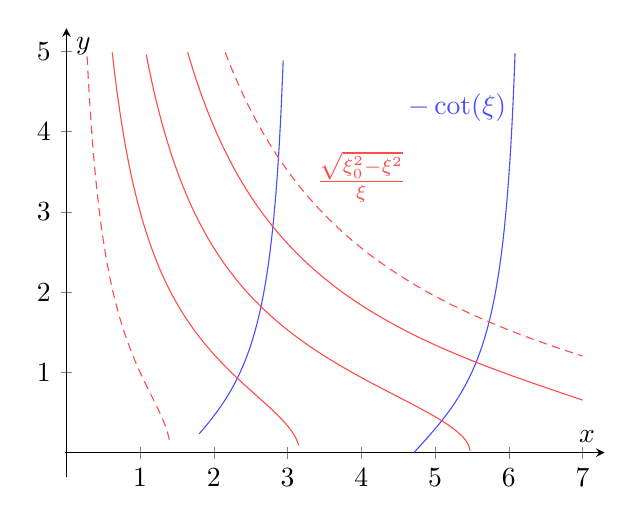
\begin{tikzpicture}
	  \begin{axis}%
	    [
	     xlabel=$x$,
	     ylabel=$y$,
	     axis lines=middle,
	     restrict y to domain=0:5.,
	     enlargelimits={abs=.3}
	    ]
	\addplot+[mark=none, 
	    domain=4.2:6.5,
	    samples=350,
	    draw=blue!70,
	    area legend] {-cot(deg(x))}  ;
	    \node [above, color=blue!70] at (5.3, 4.) {$-\cot(\xi)$};
	\addplot+[mark=none, 
	    domain=1.8:3.5,
	    samples=350,
	    draw=blue!70,
	    area legend] {-cot(deg(x))}  ;
	    \node [above, color=red!70] at (3, 0.6) {};
	\addplot+[mark=none, 
	    domain=0:7,
	    samples=350,
	    draw=red!70,
	    area legend] {sqrt(10 - x^2)/x}  ;
	    \node [above, color=red!70] at (3, 0.6) {};
	\addplot+[mark=none, 
	    domain=0:7,
	    samples=350,
	    draw=red!70,
	    area legend] {sqrt(30 - x^2)/x}  ;
	    \node [above, color=red!70] at (3, 0.6) {};
	\addplot+[mark=none, 
	    domain=0:7,
	    samples=350,
	    draw=red!70,
	    area legend] {sqrt(70 - x^2)/x}  ;
	    \node [above, color=red!70] at (3, 0.6) {};
	\addplot+[mark=none, 
	    domain=0:7,
	    samples=950,
	    draw=red!70,
	    area legend] {sqrt(120 - x^2)/x}  ;
	    \node [above, color=red!70] at (4, 3.) {$ \frac{\sqrt{\xi_0^2 - \xi^2}}{\xi}$};
	\addplot+[mark=none, 
	    domain=0:7,
	    samples=350,
	    draw=red!70,
	    area legend] {sqrt(2 - x^2)/x}  ;
	    \node [above, color=red!70] at (3, 0.6) {};  \end{axis}
	\end{tikzpicture}
         \label{fig:cos}
     \end{subfigure}
     \hspace{3cm}
     \begin{subfigure}[b]{0.4\linewidth}
         \centering
	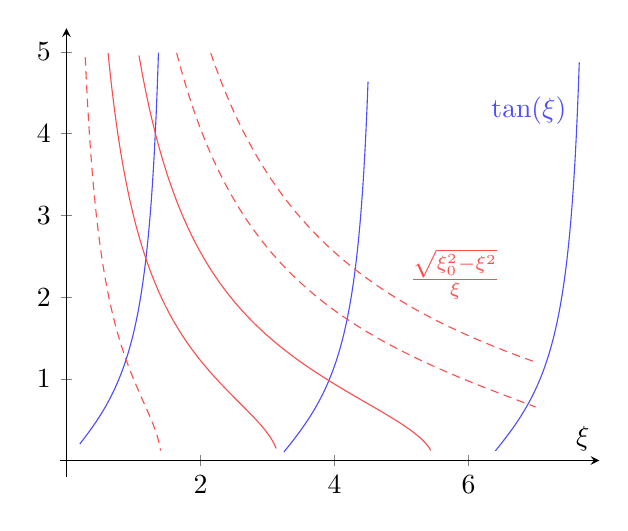
\begin{tikzpicture}
	\begin{axis}%
	[
	xlabel=$\xi$,
	axis lines=middle,
	restrict y to domain=0.1:5.,
	enlargelimits={abs=.3}
	]
	\addplot+[mark=none, 
	    domain=6.4:8.5,
	    samples=350,
	    draw=blue!70,
	    area legend] {tan(deg(x))}  ;
	    \node [above, color=blue!70] at (6.9, 4.) {$\tan(\xi)$};
	\addplot+[mark=none, 
	    domain=3.2:4.5,
	    samples=350,
	    draw=blue!70,
	    area legend] {tan(deg(x))}  ;
	    \node [above, color=red!70] at (3, 0.6) {};
	\addplot+[mark=none, 
	    domain=0.2:2.5,
	    samples=350,
	    draw=blue!70,
	    area legend] {tan(deg(x))}  ;
	    \node [above, color=red!70] at (3, 0.6) {};
	\addplot+[mark=none, 
	    domain=0:7,
	    samples=350,
	    draw=red!70,
	    area legend] {sqrt(10 - x^2)/x}  ;
	    \node [above, color=red!70] at (3, 0.6) {};
	\addplot+[mark=none, 
	    domain=0:7,
	    samples=350,
	    draw=red!70,
	    area legend] {sqrt(30 - x^2)/x}  ;
	    \node [above, color=red!70] at (3, 0.6) {};
	\addplot+[mark=none, 
	    domain=0:7,
	    samples=350,
	    draw=red!70,
	    area legend] {sqrt(70 - x^2)/x}  ;
	    \node [above, color=red!70] at (3, 0.6) {};
	\addplot+[mark=none, 
	    domain=0:7,
	    samples=950,
	    draw=red!70,
	    area legend] {sqrt(120 - x^2)/x}  ;
	    \node [above, color=red!70] at (5.8, 1.85) {$ \frac{\sqrt{\xi_0^2 - \xi^2}}{\xi}$};
	\addplot+[mark=none, 
	    domain=0:7,
	    samples=350,
	    draw=red!70,
	    area legend] {sqrt(2 - x^2)/x}  ;
	    \node [above, color=red!70] at (3, 0.6) {};
	\end{axis}
	\end{tikzpicture}
         \label{fig:puls}
     \end{subfigure}
        \caption{De transcendentale ligningene som bestemmer energien til partikkel i boks.}
        \label{fig:trans}
\end{figure}
Vi ser at vi bare for noen tillate løsninger for en gitt verdi av $\xi_0$. Når vi øker $\xi_0$, 
dvs øker $V_0$, $a$ eller $m$ så får vi flere mulige bundne ($E<V_0$) tilstander, siden det er 
da flere krysningspunkter mellom $\sqrt{\xi_0 - \xi}/\xi$ og $-\cot(\xi)$ eller $\tan(\xi)$.

Vi ser at for $V_0\to\infty$ har vi at energiene bestemmes av $\tan(\xi)=\infty$ og 
$\cot(-\xi) = \infty$, som har løsninger
\begin{align}
	 \xi = (2n+1)\frac{\pi}{2} \hspace{0.5cm}  &\land  \hspace{0.5cm} \xi = n\pi\\
	\Rightarrow E =& \frac{n^2 \pi ^2 \hbar^2}{2ma^2}
\end{align}
som er energiene vi fant for partikel i boks, hvilket vi burde forvente siden brønnen blir til en 
boks når vi sender $V_0\to\infty$, vi ser her dog også at vi får samme resultat om vi sender 
bredden til brønnen $a\to\infty$.

\begin{figure}[h!]
     \centering
     \begin{subfigure}[b]{0.4\linewidth}
       \centering
	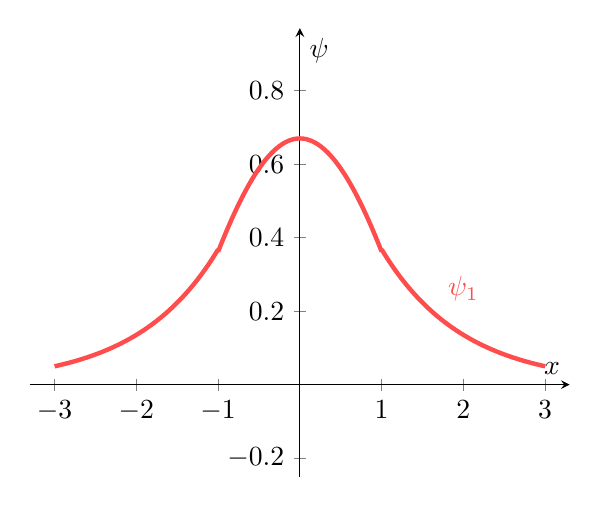
\begin{tikzpicture}
	  \begin{axis}%
	    [
	     xlabel=$x$,
	     ylabel=$\psi$,
	     axis lines=middle,
	     restrict y to domain=0:5.,
	     enlargelimits={abs=.3},
    every axis plot/.append style={ultra thick}
	    ]
	\addplot+[mark=none, 
	    domain=1:3,
	    samples=350,
	    draw=red!70,
	    area legend] {e^(-x)}  ;
	    \node [above, color=red!70] at (3, 0.6) {};
	\addplot+[mark=none, 
	    domain=-1:1,
	    samples=350,
	    draw=red!70,
	    area legend] {0.67*cos(deg(x))}  ;
	    \node [above, color=red!70] at (3, 0.6) {};
	\addplot+[mark=none, 
	    domain=-3:-1,
	    samples=350,
	    draw=red!70,
	    area legend] {e^(x)}  ;
	    \node [above, color=red!70] at (2, 0.2) {$\psi_1$};
	\end{axis}
	\end{tikzpicture}
	 \label{fig:cos}
     \end{subfigure}
     \hspace{3cm}
     \begin{subfigure}[b]{0.4\linewidth}
	 \centering
	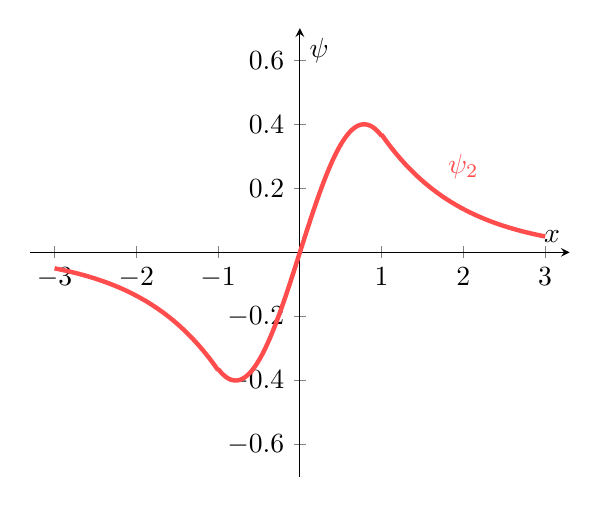
\begin{tikzpicture}
	\begin{axis}%
	[
	xlabel=$x$,
	ylabel=$\psi$,
	axis lines=middle,
	restrict y to domain=-1:1.,
	enlargelimits={abs=.3},
    every axis plot/.append style={ultra thick}
	]
	\addplot+[mark=none, 
	    domain=1:3,
	    samples=350,
	    draw=red!70,
	    area legend] {e^(-x)}  ;
	    \node [above, color=red!70] at (3, 0.6) {};
	\addplot+[mark=none, 
	    domain=-1:1,
	    samples=350,
	    draw=red!70,
	    area legend] {0.4*sin(deg(x * 2))}  ;
	    \node [above, color=red!70] at (3, 0.6) {};
	\addplot+[mark=none, 
	    domain=-3:-1,
	    samples=350,
	    draw=red!70,
	    area legend] {-e^(x)}  ;
	    \node [above, color=red!70] at (2, 0.2) {$\psi_2$};
	\end{axis}
	\end{tikzpicture}
	 \label{fig:puls}
     \end{subfigure}
	\caption{Bølgefunksjonene til partikkel i boks.}
	\label{bølgef}
\end{figure}
Vi ser fra formen til bølgefunksjonene at de tilstandene med høyere energi har større 
sannsynlighet for å befinne seg utenfor boksen. Siden Bølgefunksjonene penetrerer lenger inn 
regionen hvor $V>E$. 
de klassisk forbudte området. Igjen har vi da i ekstremtilfellet når energien er uendelig mye 
lavere enn $V_0$ at vi får igjen partikkel i boks, hvor vi så at det er umulig for partikkelen 
å befinne seg utenfor boksen.



\section*{Kvalitative betraktninger}
Vi skal nå drøfte kvalitativt oppførselen til energi egentilstander (stasjonære tilstander)
i forskjellige potensialer.
Vi har den generelle S.L. i et område hvor $E>V(x)$ som
\begin{align}
	 \frac{\partial^2 \psi}{\partial x^2} = - k^2(x) \psi
\end{align}
hvor 
\begin{align}
	 k^2(x) = \frac{2m [E - V(x)]}{\hbar^2}
\end{align}
Her ser vi at den andrederiverte har motsatt fortegn som bølgefunksjonen selv. 
Dette betyr at bølgefunksjonen alltid blyer seg inn mot x-aksen, og det betyr altså 
at bølgefunksjonen oscillerer. Dette er det samme som vi fant for partikkel i boks og brønn, men 
vi ser her at det gjelder helt generelt i områder hvor energien er større en potensialet.

Videre ser vi for oss et område med $E< V(x)$, hvor vi nå har
\begin{align}
	 \frac{\partial^2 \psi}{\partial x^2} =  \kappa^2(x) \psi
\end{align}
hvor
\begin{align}
	 \kappa^2(x) = \frac{2m [V(x) - E]}{\hbar^2}
\end{align}
Her ser vi at den andrederiverte har samme fortegn som bølgefunksjonen selv. Hvilket forteller 
oss at i områder hvor energien er mindre en potensialet så krummer alltid bølgefunksjonen vekk 
vekk fra x-aksen.

Vi ser her da at vi ikke kan ha en normaliserbar bølgefunksjon hvis vi har $V(x)>E$ for alle $x$,
vi trenger områder med $E >V(x)$ for å kunne ha en normaliserbar stasjonær tilstand.
Slik var det med partikkel i brønn hvor bølgefunksjon krummet vekk ($V(x) > E$) 
ifra x-aksen til høyre og 
venstre for brønnen mens den oscillererte ($V(X) <E$) inne i brønnen.
Tilsvarende kan vi ikke ha en normaliserbar stasjonær tilstand om vi har $V(x)<E$ overalt. 
Dette husker vi ifra diskusjonen rundt bølgepakken, hvor vi så at planbølgene ikke var 
normaliserbare.
\begin{figure}[h!]
     \centering
     \begin{subfigure}[b]{0.4\linewidth}
       \centering
	\begin{tikzpicture}
	  \begin{axis}%
	    [
	     xlabel=$x$,
	     ylabel=$\psi$,
	     axis lines=middle,
	     restrict y to domain=-2:2.,
	     enlargelimits={abs=.3},
    every axis plot/.append style={ultra thick}
	    ]
	\addplot+[mark=none, 
	    domain=-2.15:-1,
	    samples=350,
	    draw=red!70,
	    area legend] {sin(deg(x))}  ;
	    \node [above, color=red!70] at (1, 0.85) {$\psi$};
	\addplot+[mark=none, 
	    domain=1:2.15,
	    samples=350,
	    draw=red!70,
	    area legend] {sin(deg(x))}  ;
	    \node [above, color=red!70] at (-1, -0.85) {$\psi$};
	\end{axis}
	\end{tikzpicture}
	\caption{$E>V(x)$}
	 \label{fig:cos}
     \end{subfigure}
     \hspace{1cm}
     \begin{subfigure}[b]{0.4\linewidth}
	 \centering
	\begin{tikzpicture}
	\begin{axis}%
	[
	xlabel=$x$,
	ylabel=$\psi$,
	axis lines=middle,
	restrict y to domain=-3:3.,
	enlargelimits={abs=.3},
    every axis plot/.append style={ultra thick}
	]
	\addplot+[mark=none, 
	    domain=-2.15:-1,
	    samples=350,
	    draw=red!70,
	    area legend] {sin(deg(x)) + 1.25 }  ;
	    \node [above, color=red!70] at (-1, 0.4) {$\psi$};
	\addplot+[mark=none, 
	    domain=1:2.15,
	    samples=350,
	    draw=red!70,
	    area legend] {sin(deg(x)) - 1.25}  ;
	    \node [above, color=red!70] at (1, -0.35) {$\psi$};
	\end{axis}
	\end{tikzpicture}
	\caption{$E<V(x)$}
	 \label{fig:puls}
     \end{subfigure}
	\caption{Energi egentilstander for områder med forskjellige potensial-størrelser.}
	\label{bølgef}
\end{figure}


\section*{Harmonisk oscillator}

Vi skal nå se på harmonisk oscillator potensialet, 
som er et veldig viktig potensiale i kvantefysikk.
En av grunnene til at H.O. er et så viktig potensial er at det er en god tilnærming til mange 
andre potensialer rundt lokale minima.
Dette kan vi se ved å Taylor-utvikle et potensial $V(x)$ om et minima $ x_0 $ 
\begin{align}
	 V(x) = V(x_0) + \Big( \frac{\partial V}{\partial x}  \Big)_{x=x_0} (x - x_0)
	+ \frac{1}{2}\Big( \frac{\partial^2 V}{\partial x^2}  \Big)_{x=x_0} (x-x_0)^2 + \ldots 
\end{align}
Men siden $ x_0 $ er et minimum forsvinner den førster-deriverte her og vi har 
\begin{align}
	 V(x) \approx V(x_0) 
	+ \frac{1}{2}\Big( \frac{\partial^2 V}{\partial x^2}  \Big)_{x=x_0} (x-x_0)^2 
\end{align}
som en god tilnærming til potensialet når utslagene ikke er altfor store.
Vi lar 
\begin{align}
	 K = m\omega^2 = \Big( \frac{\partial^2 V}{\partial x^2}  \Big)_{x=x_0}
\end{align}
være analog til fjærkonstanten, hvor $\omega$ er angulerfrekvensen tl fj'ren.
Vi står fritt til å legge null-nivået til energien hvor vi vil, så vi lar $V(x_0)=0$.
Vi har da
\begin{align}
	 V(x) = \frac{1}{2}m\omega^2 x^2
\end{align}
Slik at vi har S.L.
\begin{align}
  \frac{\partial^2 \psi}{\partial x^2} = \frac{2m}{\hbar^2} ( \frac{1}{2}m\omega^2 x^2 - E)\psi
\end{align}
Dette er en differensialligning som er noe komplilsert å løse.
Vi starter dog med å se på tilfellet hvor utslaget er stort, slik at vi har 
\begin{align}
  \frac{\partial^2 \psi}{\partial x^2} \approx \frac{2m\omega^2}{\hbar^2}  x^2 \psi
\end{align}
Dette er forholdsvis enkelt å løse og vi har 
\begin{align}
	 \psi(x) = A x^n e^{ - \frac{m\omega x^2 }{2\hbar}} + B x^n e^{\frac{m\omega x^2 }{2\hbar}}
\end{align}
hvor vi må ha $B=0$ siden vi må ha $\psi\to 0$ når $|x|\to\infty$.
Vi kan se på tilstanden $n=0$
\begin{align}
	 \psi_0(x) = N_0 e^{- \frac{m\omega x^2}{ 2 \hbar}}
\end{align}
Dette viser seg å være den eksakte grunntilstanden for H.O. uavhengig av utslaget.
Vi setter inn i S.L. for å bekrefte dette 
\begin{align}
	 - \frac{\hbar^2}{2m} \frac{\partial^2}{\partial x^2} e^{- \frac{m\omega x^2}{ 2 \hbar}}
	+ \frac{1}{2}m\omega^2 x^2 e^{- \frac{m\omega x^2}{ 2 \hbar}} 
	&= E e^{- \frac{m\omega x^2}{ 2 \hbar}} \\
\Rightarrow - \frac{\hbar^2}{2m}( -\frac{m\omega }{\hbar} + (\frac{m\omega x}{\hbar})^2) 
 e^{- \frac{m\omega x^2}{ 2 \hbar}} + \frac{1}{2}m\omega^2 x^2 e^{- \frac{m\omega x^2}{ 2 \hbar}} 
	&= E e^{- \frac{m\omega x^2}{ 2 \hbar}} \\
\Rightarrow \frac{1}{2}\hbar\omega e^{- \frac{m\omega x^2}{ 2 \hbar}}  
	&= E e^{- \frac{m\omega x^2}{ 2 \hbar}} \\
\Rightarrow \frac{1}{2}\hbar\omega  
	&= E
\end{align}
hvor vi ser at $ \psi_0 $ er en løsning med energi $ E=\frac{1}{2}\hbar \omega $. 
Vi kan også normalisere $ \psi_0 $hvor vi har 
\begin{align}
	 1 &= \int_{-\infty}^{\infty} |N_0|^2 e^{- \frac{m\omega x^2}{\hbar}} dx\\
	  &=  |N_0|^2 \sqrt{\pi} ( \frac{m\omega}{\hbar})^{-\frac{1}{2}} \\
	\Rightarrow N_0  &=  (\frac{m\omega}{\pi\hbar})^{\frac{1}{4}}
\end{align}
slik at grunntilstanden til H.O. er 
\begin{align}
	\psi_0(x) = (\frac{m\omega}{\pi\hbar})^{\frac{1}{4}} e^{- \frac{m\omega x^2}{2\hbar}} 
\end{align}
Man kan også regne ut de alle de eksakte bølgefunksjonene til H.O. og vi har at 
\begin{align}
	 \psi_n(x) =  N_n H_n(\sqrt{ \frac{m\omega}{\hbar}} x) e^{- \frac{m\omega x^2}{2\hbar}}
\end{align}
hvor energiene er gitt som 
\begin{align}
	 E_n = (n + \frac{1}{2}) \hbar \omega
\end{align}

\subsection*{Null-punkts energien \& Heisenberg's uskarphetsrelasjon}

At det finnes en grunntilstand for H.O. som ikke har energi lik null, er interessant. Vi ser på 
forventningsverdien i Energi for grunntilstanden
\begin{align}
	 \langle E \rangle &= \int_{-\infty}^{\infty} \psi_0^* ( 
  \frac{1}{2m}(-i\hbar \frac{\partial}{\partial x}  )^2 + \frac{1}{2}m\omega^2 x^2) \psi_0 dx\\
  &= \frac{ \langle p^2 \rangle }{2m} + \frac{1}{2}m\omega^2 \langle x^2 \rangle 
\end{align}
Vi har dog at $H\psi_0 = E_0\psi_0$, og vi har at 
\begin{align}
 \langle x \rangle &= N_n \int_{-\infty}^{\infty} x e^{- \frac{m\omega x^2}{2\hbar}} dx = 0
\end{align}
og 
\begin{align}
    \langle p \rangle &= N_n \int_{-\infty}^{\infty} ( -i\hbar \frac{\partial}{\partial x} )
   e^{- \frac{m\omega x^2}{2\hbar}} dx\\
  &=  i m\omega N_n \int_{-\infty}^{\infty}x e^{- \frac{m\omega x^2}{2\hbar}} dx = 0 
\end{align}
hvor vi har brukt symmetribetraktninger.
Dette gir oss at 
\begin{align}
	 (\Delta x)^2 &= \langle x^2 \rangle \\
	 (\Delta p)^2 &= \langle p^2 \rangle 
\end{align}
Slik at vi har 
\begin{align}
	 E_0 = \frac{(\Delta p^2)}{2m} + \frac{1}{2} m\omega^2 (\Delta x^2)
\end{align}
Men nå kan vi bruke Heisenberg's uskarphetsrelasjon $\Delta x \Delta p \ge \hbar / 2$.
Vi bruker nå at $2 \Delta x / \hbar \ge 1 / \Delta p$.
Vi har nå
\begin{align}
	 E_0 \ge \frac{\hbar^2}{8 m (\Delta x)^2} + \frac{1}{2}m\omega^2 (\Delta x)^2
\end{align}
Dette må holde for grunntilstands energien, vi vet at naturen alltid vil være i den minst 
energetiske tilstanden. Vi finner minima for energien da ved å derivere mhp.  $ \Delta x $ og 
sette lik 0. Dett gir oss
\begin{align}
	 - \frac{\hbar^2}{4m (\Delta x)^3} + m\omega^2 \Delta x = 0
\end{align}
som leder til 
\begin{align}
	 (\Delta x)^2 = \frac{\hbar}{2m\omega}
\end{align}
Som vi setter inn i uttrykket vårt for $E_0$ og finner 
\begin{align}
	 E_0 \ge \frac{1}{4}\hbar \omega \frac{1}{4}\hbar \omega = \frac{1}{2}\hbar \omega
\end{align}
Dette er den minste energien som er forenelig med Heisenberg's uskarphetsrelasjon, og vi kjenner
det igjen som den faktiske grunntilstanden til H.O. Vi har da at den Gaussiske grunntilstanden 
er en minimum uskarphets-tilstand.
Dette er i sterk kontrast til den klassiske H.O., hvor vi vet at grunntilstanden har energi lik 
null og partikkelen bare sitter stille ved $x=0$. 
Dette bryter dog med Heisenberg's uskarphetsprinsipp siden vi da ville ha kjent posisjon
og bevegelsesmengde skarpt samtidig.

I kvantefysikk har H.O. grunntilstanden en lik miks av forventningsverdi som kommer 
fra potensiell og kinetisk energi, i motsetning til klassisk hvor det bare er potensiell energi
i grunntilstanden.

Denne framgangsmåten med å bruke Heisenberg's uskarphetsprinsipp for å beregne 
grunntilstandsenergien virket så bra fordi potensialet går som $x^2$. For andre potensialer kan 
man også bruke Heisenberg uskarphetsprinsipp for å beregne energien i grunntilstanden men man må 
da typisk ty til approksimasjoner.




\section*{Dirac delta funksjon potensialet}
Vi skal nå betrakte et potensiale beskrevet ved Dirac delta funksjonen, som strengt tatt ikke 
er en funksjon (matematisk sett), det er heller en grense av en sekvens med funksjoner.
Vi kan definere det som 
\begin{align}
	 \delta(x) = \lim_{b\to\infty} \sqrt{ \frac{b}{\pi} } e^{-bx^2}
\end{align}
hvor vi ser at Dirac deltaet er normalisert 
\begin{align}
	 \int_{-\infty}^{\infty}  \delta(x) dx &= 
	\lim_{b\to\infty} \sqrt{ \frac{b}{\pi} } \int_{-\infty}^{\infty} e^{-bx^2} dx \\
	 &= \lim_{b\to\infty} \sqrt{ \frac{b}{\pi} } \sqrt{ \frac{\pi}{b}} = 1
\end{align}
Vi har at i grensen $b\to\infty$ får vi 
\begin{align}
	 \delta(x) = \begin{cases}
		0 \hspace{1cm} x\neq 0 \\
		\infty \hspace{0.85cm} x = 0
		\end{cases}
\end{align}
Typisk dukker Dirac delta opp inne i integrander. Vi har da at 
\begin{align}
 \int_{-\infty}^{\infty} f(x) \delta(x)  dx = f(0) \int_{-\infty}^{\infty} \delta(x)dx = f(0)
\end{align}
hvor $ f(x) $ er en hvilket som helst godt oppført funksjon.

Vi ser nå for oss et potensial som er null overalt bortsett fra i origo, det kan vi skrive som 
\begin{align}
	 \frac{2m}{\hbar^2} V(x) = - \frac{\alpha}{a} \delta(x)
\end{align}
hvor vi merker oss at $ \frac{2m}{\hbar^2} $ har dimensjoner $ \frac{1}{\text{lengde}^2} $. Siden 
delta-funksjonen har dimension $ \frac{1}{\text{lengde}} $ må vi da ha med konstanten $\frac{\alpha}{a}$ hvor $\alpha$ er dimensionsløs og $a$ har dimensjon lengde. Vi kan nå variere $\alpha$ for 
å justere styrken på potensialet.

Vi  vet at vi egentlig alltid ønsker oss kontinurerlige bølgefunksjoner og deriverte av 
bølgefunksjonene. Men hvis vi ser på 
\begin{align}
 \int_{0^-}^{0^+} \frac{\partial^2 \psi}{\partial x^2}  dx &= 
\Big( \frac{\partial \psi}{\partial x} \Big)_{0^+} -
\Big( \frac{\partial \psi}{\partial x} \Big)_{0^-} \\					
&= \frac{2m}{\hbar^2} \int_{0^-}^{0^+} (V(x) - E) dx
\end{align}
hvor vi har brukt S.L. og kalkulusens fundamental teorem. Vi har videre 
\begin{align}
	 \frac{2mE}{\hbar^2} \int_{0^-}^{0^+} \psi(x) dx = 0
\end{align}
fordi bølgefunksjonen ikke kan være uendelig og integrasjonsdomenet infinitissemalt. 
Vi har videre at
\begin{align}
	 \frac{2m}{\hbar^2} \int_{0^-}^{0^+} V(x) \psi(x) dx = 
	- \frac{\alpha}{a} \int_{0^-}^{0^+} \delta(x) \psi(x) dx = - \frac{\alpha}{a} \psi(0)
\end{align}
Slik at vi har 
\begin{align}
\Big( \frac{\partial \psi}{\partial x} \Big)_{0^+} -
\Big( \frac{\partial \psi}{\partial x} \Big)_{0^-} = - \frac{\alpha}{a} \psi(0)
\label{eq:disc_wave}
\end{align}
og vi ser at at den første-deriverte av bølgefunksjonen er diskontinuerlig.
Og vi ser hvorfor bølgefunksjonen som regel er kontinurerlig og det er kun når potensialet er 
singulært at vi har diskontinuerlige bølgefunksjoner. Dette er også tilfellet for partikkel i 
boks hvor vi også hadde at potensialet gikk fra 0 til uendelig i punktet ved boksens ender.
Vi ser over at venstresiden alltid forsvinner over et infinitissemalt intervall for alle 
ikke-singulære potensialer.

Vi løser nå S.L., og vi ser at til høyre og venstre for boksen har vi S.L.
\begin{align}
	 \frac{\partial^2 \psi}{\partial x^2} = \frac{-2mE}{\hbar}\psi
\end{align}
Vi ønsker bundne tilstander, dvs $E<0$ og at partikkelen holder seg i nerheten av dirac deltaet.
Vi definerer derfor
\begin{align}
	 \kappa = \frac{\sqrt{-2mE}}{\hbar}
\end{align}
So gir på begge sidene av $x=0$
\begin{align}
	 \psi(x) = A e^{\kappa x} + B e^{\kappa x}
\end{align}
hvor vi må se bort ifra de potensialene divergerer når $x\to\infty$ som da gir 
\begin{align}
	 \psi(x) = \begin{cases}
		Ae^{-i\kappa x} \hspace{1cm} x \le 0 \\
		Ae^{i\kappa x} \hspace{1.2cm} x \ge 0 
		\end{cases}
\end{align}
Vi setter in for bølgefunksjonen i betingelsen for diskontinuerlighet av bølgefunksjonens 
deriverte i Lign.~\ref{eq:disc_wave} og finner
\begin{align}
	 -2\kappa A &= -\frac{\alpha}{a}A \\
	\Rightarrow \frac{\sqrt{-2mE}}{\hbar} &= \frac{\alpha}{2 a} \\
	\Rightarrow E &= - \frac{\alpha^2 \hbar^2}{8 m a^2}
\end{align}
Vi har bare en bundet tilstand for Dirac delta potensialet. Dette kunne vi også ha sett utifra 
våre kvalitative betraktninger om bølgefunksjonens krumning, hvor vi ser at bølgefunksjonen 
må ha positiv andre-derivert overalt, og i tilleg være kontinuerlig. Da er det bare en mulig 
bølgefunksjon som kan oppfylle dette. Dette burde vi kanskje også forvente utifra det vi så 
om partikkel i brønn, hvor vi fant at samme hvor stor eller dyb brønnen var, vil den alltid ha 
minst en bundet tilstand.

\section*{Dobbelt brønn og molekylærbinding}

Vi har sett at vi kan se for oss potensialbrønnen som representativ for et elektron
fanget av e.g. et Hydrogen atom, hvor potensialbrønnen befinner seg rundt protonet. 
Veien er kort derfra til å se for seg at vi kan bruke to potensialbrønner til å beskrive 
molekylærbinding til e.g. et H$^+_2$ ion.
Vi kan bruke det til å se på hvorfor molekylær overhodet kan eksistere.
\begin{figure}[h!]
     \centering
     \begin{subfigure}[b]{0.4\linewidth}
       \centering
	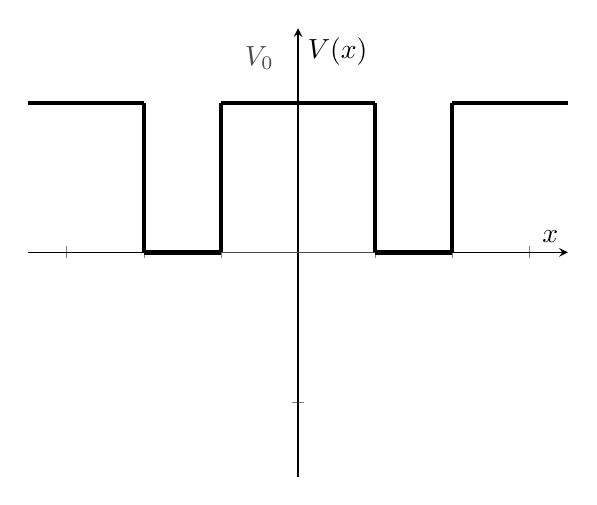
\begin{tikzpicture}
	  \begin{axis}%
	    [
	     xlabel=$x$,
	     ylabel=$V(x)$,
	     axis lines=middle,
	     restrict y to domain=-1:2.,
	     enlargelimits={abs=.75},
	     yticklabels=\empty,
	     xticklabels=\empty
	    ]
	    \addplot+[mark=none, 
		    domain=-1:1,
		    samples=150,
		    draw=black!70,
		    pattern color=black,
	    	    area legend] { 0 }  ;
	    \node [color=black!70] at (-0.25, 0.65) {$V_0$};
	\draw [ultra thick] (1, 0.5) -- (2,0.5);
	\draw [ultra thick] (-1, 0.5) -- (-2,0.5);
	\draw [ultra thick] (1, 0) -- (1,0.5);
	\draw [ultra thick] (-1, 0) -- (-1,0.5);
	\draw [ultra thick] (-1, 0.) -- (-0.5,0);
	\draw [ultra thick] (1, 0.) -- (0.5,0);
	\draw [ultra thick] (-0.5, 0) -- (-0.5,0.5);
	\draw [ultra thick] (0.5, 0) -- (0.5,0.5);
	\draw [ultra thick] (0.5, 0.5) -- (-0.5,0.5);
	  \end{axis}
	\end{tikzpicture}
         \label{fig:cos}
     \end{subfigure}
       \caption{Potensialet $V(x)$ til dobelt brønn.}
        \label{fig:bølger}
\end{figure}


Vi kan see kvalitativt på hvordan bølgefunksjonen ser ut for dobbel-brønnpotensialet.
Igjen har vi at bølgefunksjonen er oscillatorisk inne i brønnen og eksponensiell utenfor.
Vi har også at potensialet er symmetrisk $V(-x) = V(x)$ og derfor vil også bøglefunksjonen 
være det. Vi ser da at dette vil føre til at sannsynligeten for å finne elektronet er like 
stor i begge brønnene, altså ved begge protonene. Denne elektron-delingen er det som gjør 
at slike molekyler er stabile. 
Det er energetisk fordelaktig å dele på elektronet. Dette er litt knotete å regne ut dette nøyaktig
siden vi får 8 randbetingelser vi må ta hensyn til. Vi ser derfor istedet på et enklere system 
som beskriver det samme konseptet.

Vi ser på en dobbel Dirac delta potensial.

\begin{align}
	 \frac{2m}{\hbar^2} V(x) = - \frac{\alpha}{a} [\delta(x+a) - \delta(x-a)]
\end{align}
hvor vi igjen har 
\begin{align}
	 \psi(x) = A e^{-\kappa x} + Be^{\kappa x}
\end{align}
i både til høyre og venstre og imellom brønnene. I mellom brønnene trenger vi ikke forkaste  noen
av leddene siden vi ikke har $x\to\infty$ her. Dette gir en symmetrisk
\begin{align}
	 \psi_{sym}(x) = \begin{cases} 
		A e^{\kappa x} \hspace{1.7cm}  x\le -a \\
		B \cosh(\kappa x) \hspace{0.85cm} x \in [-a, a] \\
		A e^{-\kappa x} \hspace{1.5cm}  x\ge a 
		\end{cases}
\end{align}
og en asymmetrisk
\begin{align}
	 \psi_{asym}(x) = \begin{cases} 
		A e^{\kappa x} \hspace{1.7cm}  x\le -a \\
		B \sinh(\kappa x) \hspace{0.85cm} x \in [-a, a] \\
		-A e^{-\kappa x} \hspace{1.5cm}  x\ge a 
		\end{cases}
\end{align}
bølgefunksjon, hvor vi minner om at vi har 
\begin{align}
	 \cosh(x) &= \frac{e^{x} + e^{-x}}{2}\\
	 \sinh(x) &= \frac{e^{x} - e^{-x}}{2} \\
	 \tanh(x) &= \frac{\sinh(x)}{\cosh(x)} = \frac{e^{x} - e^{-x}}{e^{x} + e^{-x}} \\
\end{align}

\subsubsection*{Symmetrisk}
Vi ser at bølgefunksjonen er symmetrisk rundt origo $\psi(-x) = \psi(x)$. 
Vi får nå at kontinuerlighet av bølgefunksjonen gir at vi må ha 
\begin{align}
	 B\cosh(\kappa x) = A e^{-\kappa x}
\end{align}
og betingelsen for diskontinuerligheten for den første deriverte ved brønnen e.g. til høyre gir
\begin{align}
\Big( \frac{\partial \psi}{\partial x} \Big)_{a^+} -
\Big( \frac{\partial \psi}{\partial x} \Big)_{a^-} &= - \frac{\alpha}{a} \psi(a) \\
\Rightarrow - \kappa A  e^{-\kappa a}  -\kappa B \sinh(\kappa a) 
				&= -\frac{\alpha}{a} B \cosh(\kappa a)\\
\Rightarrow  -\kappa B\cosh(\kappa a) -\kappa B \sinh(\kappa a) 
				&= -\frac{\alpha}{ a} B \cosh(\kappa a) \\
\Rightarrow  -1 -\tanh(\kappa a)  &= -\frac{\alpha}{\kappa a}  \\
\Rightarrow  \tanh(\kappa a)  &= \frac{\alpha}{\kappa a}  - 1
\end{align}
hvor vi har brukt betingelsen for kontinuerlighet av bølgefunksjonen.
\begin{figure}[h!]
	\centering
      \begin{subfigure}[b]{0.4\linewidth}
       \centering
	\begin{tikzpicture}
	  \begin{axis}%
	    [
	     xlabel=$\kappa a$,
	     %ylabel=$$,
	     axis lines=middle,
	     restrict y to domain=-1:2.,
	     enlargelimits={abs=.5},
	     yticklabels=\empty,
	     xticklabels=\empty,
    	every axis plot/.append style={ thick}
	    ]
	    \addplot+[mark=none, 
		    domain=0:3,
		    samples=150,
		    draw=red!70,
	    	    area legend] { 3 / x - 1 }  ;
	    \addplot+[mark=none, 
		    domain=0:3,
		    samples=550,
		    draw=blue!70,
	    	    area legend] { tanh( x ) }  ;
	    \node [color=black!70] at (-0.15, 1) {$1$};
	    \node [color=red!70] at (1.6, 1.7) {$\frac{\alpha}{\kappa a} - 1$};
	    \node [color=blue!70] at (2.6, 0.75) {$\tanh(\kappa a)$};
	    \draw[dashed] (0,1) -- (5,1);
	  \end{axis}
	\end{tikzpicture}
         \caption{Symmetrisk bølgefunksjon}
     \end{subfigure}
     \hspace{1cm}
     \begin{subfigure}[b]{0.4\linewidth}
       \centering
	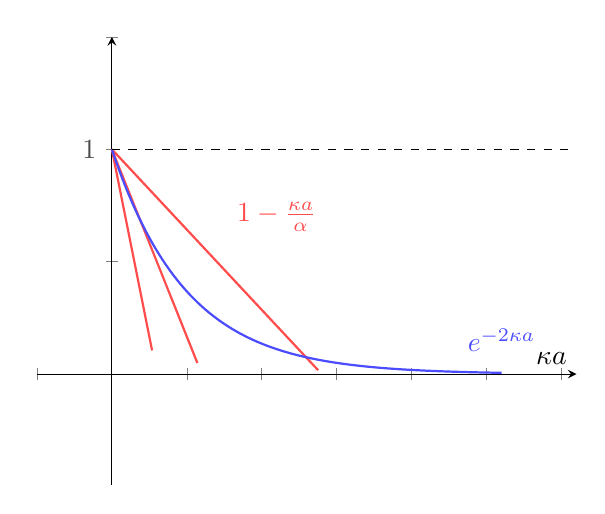
\begin{tikzpicture}
	  \begin{axis}%
	    [
	     xlabel=$\kappa a$,
	     %ylabel=$$,
	     axis lines=middle,
	     restrict y to domain=-0.:5.,
	     enlargelimits={abs=.5},
	     yticklabels=\empty,
	     xticklabels=\empty,
    	every axis plot/.append style={ thick}
	    ]
	    \addplot+[mark=none, 
		    domain=0:5,
		    samples=150,
		    draw=red!70,
	    	    area legend] { 1 - x / 0.3 }  ;
	    \addplot+[mark=none, 
		    domain=0:5,
		    samples=150,
		    draw=red!70,
	    	    area legend] { 1 - x / 1.4 }  ;
	    \addplot+[mark=none, 
		    domain=0:5,
		    samples=150,
		    draw=red!70,
	    	    area legend] { 1- x / 0.6  }  ;
	    \addplot+[mark=none, 
		    domain=0:2.6,
		    samples=550,
		    draw=blue!70,
	    	    area legend] { exp( -2*x ) }  ;
	    \node [color=black!70] at (-0.15, 1) {$1$};
	    \node [color=red!70] at (1.1, 0.7) {$1-\frac{\kappa a}{\alpha}$};
	    \node [color=blue!70] at (2.6, .15) {$e^{-2\kappa a}$};
	    \draw[dashed] (0,1) -- (5,1);
	  \end{axis}
	\end{tikzpicture}
         \caption{asymmetrisk bølgefunksjon}
     \end{subfigure}
       \caption{Transcendental ligning for energien i til dobbel Dirac delta 
       potensial.}
        \label{fig:bølger}
\end{figure}
Vi vet at $\tanh(\kappa a)$ alltid er mindre enn 1 siden tangens hyperbolicus funksjonen er 
begrenset. 
Dette gir da 
\begin{align}
	 \frac{\alpha}{\kappa a} - 1 &< 1 \\
\Rightarrow \kappa &< \frac{\alpha}{2a} \\
\Rightarrow E &< -\frac{\hbar^2 \alpha^1}{8ma^2}
\end{align}

\subsubsection*{Asymmetrisk}
Vi ser nå på den asymetriske bølgefunksjonen rundt origo $\psi(-x) = -\psi(x)$. 
Vi får nå at kontinuerlighet av bølgefunksjonen i dette tilfellet ved $x=a$ gir
\begin{align}
	 B\sinh(\kappa x) = -A e^{-\kappa x}
\end{align}
og betingelsen for diskontinuerligheten for den første deriverte ved brønnen e.g. til høyre gir
\begin{align}
\Big( \frac{\partial \psi}{\partial x} \Big)_{a^+} -
\Big( \frac{\partial \psi}{\partial x} \Big)_{a^-} &= - \frac{\alpha}{a} \psi(a) \\
\Rightarrow \kappa A  e^{-\kappa a}  - \kappa B \cosh(\kappa a) 
				&= -\frac{\alpha}{a} B \sinh(\kappa a)\\
\Rightarrow  -\kappa B\sinh(\kappa a) - \kappa B \cosh(\kappa a) 
				&= - \frac{\alpha}{ a} B \sinh(\kappa a) \\
\Rightarrow  -(e^{\kappa a} - e^{-\kappa a}) - (e^{\kappa a} + e^{-\kappa a}) 
				&= - \frac{\alpha}{\kappa a} (e^{\kappa a} - e^{-\kappa a})  \\
\Rightarrow  -2e^{\kappa a} &= - \frac{\alpha}{\kappa a} (e^{\kappa a} - e^{-\kappa a})  \\
\Rightarrow   \frac{2e^{\kappa a}}{e^{\kappa a} - e^{-\kappa a}} &= \frac{\alpha}{\kappa a}  \\
\Rightarrow   \frac{1}{1 - e^{-2\kappa a}} &= \frac{\alpha}{2\kappa a}  \\
\Rightarrow   e^{-2\kappa a} &= 1 - \frac{2\kappa a}{\alpha}
\end{align} 
hvor vi har brukt betingelsen for kontinuerlighet av bølgefunksjonen.

Vi har nå funnet den transcendentale ligningen for energinivåer for den asymmetriske 
bølgefunksjon.
Vi ser at vi trenger å ha at H.S. stiger fortere en $ e^{-2\kappa a} $ ved $\kappa a=0$ for at 
ligningen har en løsning.
Vi ser derfor på stigningstallene gitt ved de deriverte ved $x=0$ av V.S.
\begin{align}
	\Big[ \frac{\partial}{\partial \kappa a} e^{-2\kappa a} \Big]_0 = 
	\Big[ -2\tanh^{-2\kappa a} \Big]_0 = -2
\end{align}
og H.S.
\begin{align}
	\Big[ \frac{\partial }{\partial \kappa a}  ( 1 - \frac{2\kappa a }{\alpha} ) \Big]_0 
	= -\frac{2}{\alpha}
\end{align}
Vi har da følgende krav for at det finnes asymmetriske bundne tilstander
\begin{align}
	 -\frac{2}{\alpha} < -2 \\
	\Rightarrow \alpha > 1 \\
\end{align}
hvor vi da ser at vi bare har en bundet tilstand med asymmetrisk bølgefunksjon og bare når 
 $\alpha > 1$. Hvis $\alpha < 1$ har vi kun en bundet tilstand, nemlig den symmetriske, siden
potensialet ikke er sterkt nok til å holde på mer energetiske tilstander.


\subsubsection*{Molekyler}
Hvor vi ser at et elektrons energi er mindre hvis det er bundet i en dobbeltbrønn en om det er 
bundet i en enkeltbrønn.
Dette er grunnen til at molekylær dannes og at vi ikke bare har atomer.
Dette er noe som går igjen i flere sammenhenger, og det at bølgefunksjonen til elektroner kan 
være på flere atomer samtidig gjør at det er energetisk fordelaktig for elektroner å slå seg 
sammen til molekyler.


\section*{Spredning og trinnpotensialet}

Vi har til nå sett på tilstander som har vært bundne, til forskjellige potensialer.
Vi skal nå igjen se på løsninger av S.L. hvor partikkelen ikke er bundet, slik som var tilfellet
for den frie S.L. Vi vil da igjen se at vi ikke får noen føringer på tillatte energier, og vi 
finner et kontinium av energier.
Vi har da at vi må overlagre løsninger fra kontiniumet av S.L. elementære løsninger med 
forskjellige energier for å lage 
en lokalisert og normaliserbar bølgepakke som er en fysikalsk tillatt bølgefunksjon.
Bølgepakken består av løsninger med forskjellige energier så den vil utvikle seg i tid, og vi 
ser nå på hvordan slike løsninger utvikler seg i tid når de treffer potensialer. Vi kaller 
vi spredning når ikke-bundne tilstander's tidsuvikling betraktes.
\begin{figure}[h!]
     \centering
     \begin{subfigure}[b]{0.4\linewidth}
       \centering
	\begin{tikzpicture}
	  \begin{axis}%
	    [
	     xlabel=$x$,
	     ylabel=$V(x)$,
	     axis lines=middle,
	     restrict y to domain=-1:2.,
	     enlargelimits={abs=.75},
	     yticklabels=\empty,
	     xticklabels=\empty
	    ]
	    \addplot+[mark=none, 
		    domain=-1:1,
		    samples=150,
		    draw=black!70,
		    pattern color=black,
	    	    area legend] { 0 }  ;
	    \node [color=black!70] at (-0.25, 0.35) {$V_0$};
	    \node [color=black!70] at (-1.2, 0.25) {$E$};
	\draw [<->] (-1, 0.025) -- (-1, 0.475);
	\draw [ultra thick] (-2, 0) -- (0, 0);
	\draw [ultra thick] (0, 0.) -- (0, 0.35);
	\draw [ultra thick] (0, 0.35) -- (2, 0.35);
	\draw [thick, dashed] (-2, 0.5) -- (2, 0.5);
	  \end{axis}
	\end{tikzpicture}
         \label{fig:cos}
     \end{subfigure}
       \caption{Trinnpotensialet $V(x)$  til en som en partikkel spredes på.}
        \label{fig:bølger}
\end{figure}


Vi starter med å betrakte 
\begin{align}
	 V(x) = \begin{cases}
		0 \hspace{1.2cm} x < 0 \\
		V_0 \hspace{1cm} x > 0
		\end{cases}
\end{align}
Nå antar vi at energien er større en potensial-barrieren $ E > V_0 $.
Vi har da S.L. 
\begin{align}
 \frac{\partial^2 \psi}{\partial x^2} &= -\frac{2mE}{\hbar^2} \psi \hspace{2.1cm} x < 0 \\
 \frac{\partial^2 \psi}{\partial x^2} &= -\frac{2m(E-V_0)}{\hbar^2} \psi \hspace{1cm} x > 0
\end{align}
hvor vi definerer
\begin{align}
	 k &= \frac{\sqrt{2mE}}{\hbar} \\
	 k_0 &= \frac{\sqrt{2m(E-V_0)}}{\hbar} 
	= \sqrt{ k^2 - \frac{2mV_0}{\hbar^2}} 
\end{align}
Vi finner da løsningene 
\begin{align}
	 \psi(x) = 
	\begin{cases}
		Ae^{ikx} + Be^{-ikx} \hspace{1.2cm} x<0 \\
	 Ce^{ik_0 x} + De^{-ik_0 x} \hspace{1cm} x>0
	\end{cases}
\end{align}
Dette er ikke normaliserbart så vi kan ikke bruke normaliseringskravet for å bestemme konstantene,
det vi istedenfor gjør er å se på sannsynlighetsstrømmen
\begin{align}
 j(x) = \frac{\hbar}{2mi}\big(\psi^* \frac{\partial}{\partial x}\psi 
 - \psi \frac{\partial}{\partial x}\psi^*   \big)
\end{align}
som for vår bølgefunksjon blir 
\begin{align}
	 j(x) = \begin{cases}
		\frac{\hbar k}{m} (|A|^2 - |B|^2) \hspace{1.15cm} x < 0 \\
		\frac{\hbar k_0}{m} (|C|^2 - |D|^2) \hspace{1.cm} x > 0 
		\end{cases}
\end{align}
Her ser vi at de positive leddene represneterer sannsynlighetsstrøm mot høyyre langs x-aksen,
og de negative leddene til venstre, og vi ser at sannsynlighetsstrømmen beveger seg med 
hastighet som er gitt ved farten til partikkelen i det mediumet den befinner seg i. 
Vi ser her også at vi må sette $D=0$, det er fordi dette representerer en sannsynlighetsstrøm 
som kommer inn fra høyre mot trinnpotensialet og det er ikke dette vi ønsker å se på. Vi vil 
betrakte en som kommer fra venstre og spres på potensial trinnet.
\begin{figure}[h!]
     \centering
     \begin{subfigure}[b]{0.4\linewidth}
       \centering
	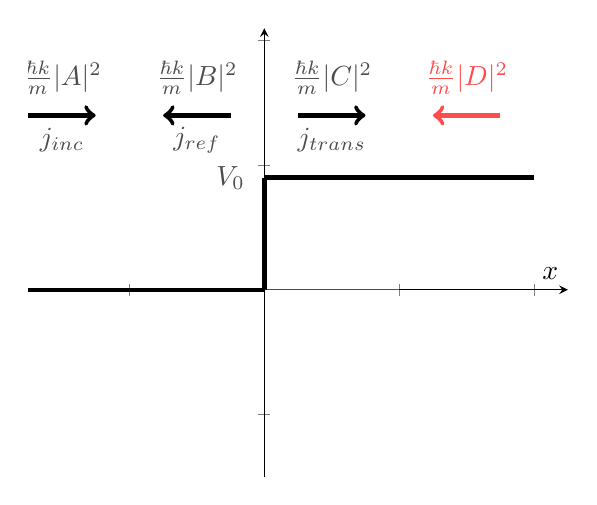
\begin{tikzpicture}
	  \begin{axis}%
	    [
	     xlabel=$x$,
	     %ylabel=$V(x)$,
	     axis lines=middle,
	     restrict y to domain=-1:2.,
	     enlargelimits={abs=.75},
	     yticklabels=\empty,
	     xticklabels=\empty
	    ]
	    \addplot+[mark=none, 
		    domain=1:1.5,
		    samples=150,
		    draw=white,
	    	    area legend] { 0.3 }  ;
	    \addplot+[mark=none, 
		    domain=-1:1,
		    samples=150,
		    draw=black!70,
		    pattern color=black,
	    	    area legend] { 0 }  ;
	    \node [color=black!70] at (-0.25, 0.45) {$V_0$};
	    \node [color=black!70] at (-0.5, 0.85) {$\frac{\hbar k}{m}|B|^2 $};
	    \node [color=black!70] at (-1.5, 0.85) {$\frac{\hbar k}{m}|A|^2 $};
	    \node [color=black!70] at (0.5, 0.85) {$\frac{\hbar k}{m}|C|^2 $};
	    \node [color=black!70] at (-0.5, 0.6) {$j_{ref}$};
	    \node [color=black!70] at (-1.5, 0.6) {$j_{inc}$};
	    \node [color=black!70] at (0.5, 0.6) {$j_{trans}$};
	    \node [color=red!70] at (1.5, 0.85) {$\frac{\hbar k}{m}|D|^2 $};
	\draw[<-, ultra thick] (-0.75, 0.7) -- (-0.25, 0.7);
	\draw[->, ultra thick] (-1.75, 0.7) -- (-1.25, 0.7);
	\draw[<-, ultra thick] (0.75, 0.7) -- (0.25, 0.7);
	\draw[->, ultra thick, red!70] (1.75, 0.7) -- (1.25, 0.7);
	\draw [ultra thick] (-2, 0) -- (0, 0);
	\draw [ultra thick] (0, 0.) -- (0, 0.45);
	\draw [ultra thick] (0, 0.45) -- (2, 0.45);
	  \end{axis}
	\end{tikzpicture}
         \label{fig:cos}
     \end{subfigure}
       \caption{sannsynlighetsstrømmen til en partikkel som spres på et trinn potensiale.}
        \label{fig:bølger}
\end{figure}
Vi definerer refleksjons og transmisjonskoeffisientene som
\begin{align}
 R &= \frac{j_{ref}}{j_{inc}} = \frac{\frac{\hbar k}{m} |B|^2}{\frac{\hbar k}{m} |A|^2} =
  \frac{ |B|^2}{|A|^2} \\
 T &= \frac{j_{trans}}{j_{inc}} = \frac{\frac{\hbar k_0}{m} |C|^2}{\frac{\hbar k}{m} |C|^2} 
 \frac{j_{trans}}{j_{inc}} = \frac{ k_0 |C|^2}{k |A|^2} 
\end{align}
Vi ser da at transmisjonskoeffisienten ikke bare er $|C|^2/|A|^2$ siden partikkelen beveger seg 
saktere i regionen til høyre for trinnet ($x>0$).

Vi bruker nå kravet om at bølgefunksjonen må være kontinuerlig overalt, og spesielt ved 
$x=0$ til å finne 
\begin{align}
	 A + B = C + D
\end{align}
og kontinuitet av de første deriverte gir 
\begin{align}
	 Aik - ikB = ik_0 C - ik_0 D 
\end{align}
Vi har 2 ligninger for å bestemme 4 ukjente. Det er mange måter å oppfylle dette underbestemte 
ligningssettet. Vi valgte allerede å sette $D=0$ på fysikalsk grunnlag. Så vi får nå
\begin{align}
	 A + B &= \frac{k}{k_0}(A-B) \\
\Rightarrow k_0(A+B) &= k(A-B) \\
\Rightarrow A(k_0 - k) &= -B(k_0 + k) \\
\Rightarrow \frac{A}{B} &= \frac{k + k_0}{k - k_0} \\
\end{align}
og 
\begin{align}
	ik_0C &= ikA - ikA \frac{k - k_0}{k_0+k} \\
	k_0C(k+k_0) &= kA (k+k_0) - kA (k - k_0) \\
	k_0C(k+k_0) &= Akk_0  + A kk_0 \\
	C(k+k_0) &= 2A k  \\
	\frac{A}{C} &=  \frac{k_+k_0}{2k} 
\end{align}
Vi ser nå at vi ikke har noe krav om hvilke energier som er tillatt. Dette kommer av at vi 
har en situasjon hvor partikkelen ikke er restriktert til et avgrenset området i rommet. 
Vi får da 
\begin{align}
	 R &= \frac{(k-k_0)^2}{(k+k_0)^2} \\
	 T &= \frac{4kk_0}{(k+k_0)^2} 
\end{align}
Vi har da også
\begin{align}
	 R+T=1
\end{align}
som vi selvsagt burde ha.

\subsubsection*{Spredning av bølgepakke}

Vi har allerede sett at vi kan lage normaliserbare bølgefunksjoner som en superposisjon av 
planbølger med forskjellig energi. Vi kan her skrive det som 
\begin{align}
	 \Psi(x,t) = \begin{cases}
	&\int_{- \infty }^{ \infty}  [ A(k) e^{i(kx - \frac{E}{\hbar}t)} - 
			B(k) e^{i(kx + \frac{E}{\hbar}t)} ] dx \hspace{1cm} x<0\\
	&\int_{- \infty }^{ \infty}  C(k) e^{i(k_0x - \frac{E}{\hbar}t)} dx \hspace{3.6cm} x>0
	  \end{cases}
\end{align}
hvor vi ser at leddet med $A(k)$ og $C(k)$ er bølger som beveger seg mot høyre og $B(k)$ 
beveger seg mot venstre. 
Vi kan også beregne transmissjon og refleksjons koeffisientene ved å beregne integralene og 
finne et eksakt uttrykk for $\Psi(x,t)$ og deretter integrere $|\Psi|^2$ på høyre og venstre 
side av potensial trinnet etter partikkelen treffer potensialet.
\begin{figure}[h!]
     \centering
     \begin{subfigure}[b]{0.4\linewidth}
       \centering
	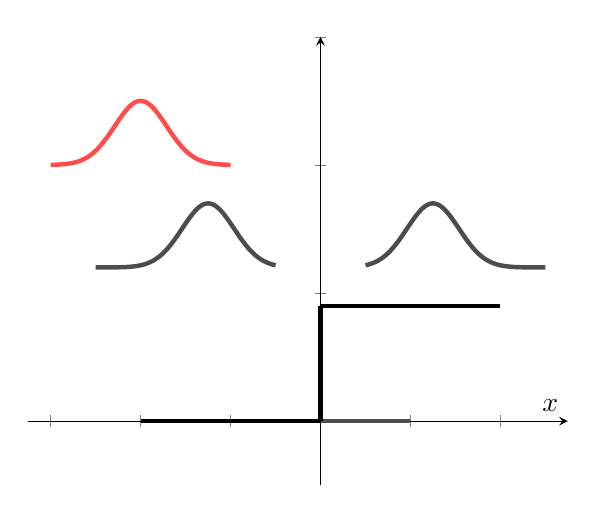
\begin{tikzpicture}
	  \begin{axis}%
	    [
	     xlabel=$x$,
	     %ylabel=$V(x)$,
	     axis lines=middle,
	     restrict y to domain=-5:5.,
	     enlargelimits={abs=.25},
	     yticklabels=\empty,
	     xticklabels=\empty,
    every axis plot/.append style={ultra thick}
	    ]
	    \addplot+[mark=none, 
		    domain=-3.:-1.,
		    samples=150,
		    draw=red!70,
	    	    area legend] { 1 + 0.25*exp(-6.*(x+2.)^2)  }  ;
	    \addplot+[mark=none, 
		    domain=-2.5:-0.5,
		    samples=150,
		    draw=black!70,
	    	    area legend] { 0.6 + 0.25*exp(-6.*(x+1.25)^2)  }  ;
	    \addplot+[mark=none, 
		    domain=2.5:0.5,
		    samples=150,
		    draw=black!70,
	    	    area legend] { 0.6 + 0.25*exp(-6.*(x-1.25)^2)  }  ;
	    \addplot+[mark=none, 
		    domain=1:1.5,
		    samples=150,
		    draw=white,
	    	    area legend] { 0.3 }  ;
	    \addplot+[mark=none, 
		    domain=-1:1,
		    samples=150,
		    draw=black!70,
		    pattern color=black,
	    	    area legend] { 0 }  ;
	\draw [ultra thick] (-2, 0) -- (0, 0);
	\draw [ultra thick] (0, 0.) -- (0, 0.45);
	\draw [ultra thick] (0, 0.45) -- (2, 0.45);
	  \end{axis}
	\end{tikzpicture}
         \label{fig:cos}
     \end{subfigure}
       \caption{sannsynlighetsstrømmen til en partikkel som spres på et trinn potensiale.}
        \label{fig:bølger}
\end{figure}



\end{document}

